\documentclass[border=10pt]{standalone}
\usepackage{pgfplots}
\pgfplotsset{compat=1.17}
\usetikzlibrary{arrows.meta}

\begin{document}
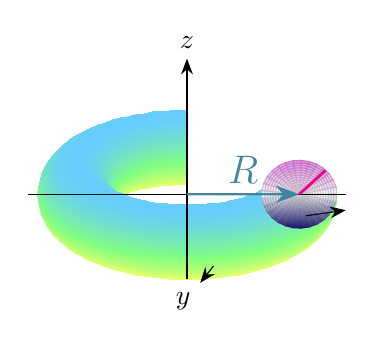
\begin{tikzpicture}
    % Define a custom colormap for the torus surface
    \pgfplotsset{
        colormap={torusmap}{
            rgb255(0cm)=(255,255,102) % Yellow
            rgb255(1cm)=(128,255,128) % Green
            rgb255(2cm)=(102,204,255) % Blue/Cyan
        },
    }

    \begin{axis}[
        hide axis,
        axis equal,
        view={-45}{25},
        xmin=-4.5, xmax=4.5,
        ymin=-4.5, ymax=4.5,
        zmin=-2.5, zmax=4,
    ]

    % Define torus parameters
    \def\majorR{3}
    \def\minorR{1}
    \def\startA{45}
    \def\endA{315}

    % Draw the main torus surface
    \addplot3[
        surf,
        shader=interp,
        colormap name=torusmap,
        domain=\startA:\endA,
        y domain=0:360,
        samples=70,
        samples y=30,
        variable=\u,
        variable y=\v,
        point meta={\minorR*sin(\v)},
        z buffer=sort,
    ] (
        {(\majorR + \minorR*cos(\v)) * cos(\u)},
        {(\majorR + \minorR*cos(\v)) * sin(\u)},
        {\minorR*sin(\v)}
    );

    % Draw the cross-section at the end
    \addplot3[
        surf,
        colormap/violet,
        domain=0:\minorR,
        y domain=0:360,
        samples=15,
        samples y=30,
        variable=\s,
        variable y=\v,
        draw=white,
        z buffer=sort,
    ] (
        {(\majorR + \s*cos(\v)) * cos(\endA)},
        {(\majorR + \s*cos(\v)) * sin(\endA)},
        {\s*sin(\v)}
    );

    % Draw the central coordinate axes
    \draw[-{Stealth[length=2mm]}] (0,0,-2.5) -- (0,0,4) node[anchor=south] {$z$};
    \draw (-3,3,0) -- (3,-3,0);
    \draw (-3,-3,0) -- (3,3,0);

    % Draw the major radius R
    \coordinate (O) at (0,0,0);
    \coordinate (C) at ({\majorR*cos(\endA)}, {\majorR*sin(\endA)}, 0);
    \draw[cyan!60!black, thick, -{Stealth[length=3mm]}] (O) -- (C) node[midway, above, sloped, font=\Large] {$R$};

    % Draw the minor radius r line on the cross-section
    \pgfmathsetmacro{\rAngleV}{45}
    \coordinate (Pr_end) at ({(\majorR+\minorR*cos(\rAngleV))*cos(\endA)}, {(\majorR+\minorR*cos(\rAngleV))*sin(\endA)}, {\minorR*sin(\rAngleV)});
    \draw[magenta, thick, line width=1pt] (C) -- (Pr_end);

    % Draw directional arrows for y and x (unlabeled)
    \draw[-{Stealth[length=2mm]}] (-1.5, -2.5, -0.8) -- (-2.5, -3.0, -0.8) node[anchor=north east] {$y$};
    \draw[-{Stealth[length=2mm]}] (2.5, -2.0, -0.8) -- (3.5, -2.5, -0.8);

    \end{axis}
\end{tikzpicture}
\end{document}